\documentclass[10pt]{book}
\usepackage{makeidx}
\usepackage{framed}
\setlength{\FrameSep}{0mm}
 
\makeindex
%\usepackage{showidx}
% mark overful hboxes
%\overfullrule=5mm
\usepackage{kpfonts}

\newcommand{\eq}{=}

%\usepackage[nott]{kpfonts}
%\SetMathAlphabet{\mathtt}{normal}{OT1}{\ttdefault}{m}{n}
%\SetMathAlphabet{\mathtt}{bold}{OT1}{\ttdefault}{m}{n}

%\usepackage[math]{iwona}
%\SetMathAlphabet{\mathtt}{iwona}{OT1}{\ttdefault}{m}{n}
%\usepackage[T1]{fontenc}

\usepackage{amsopn}
\usepackage{amsmath}
\usepackage{amsthm}
\usepackage{url}
\usepackage{graphicx}
\usepackage{datetime}
\usepackage{amsfonts}
\usepackage{graphicx}
\usepackage{threeparttable}
\usepackage{wasysym}
\usepackage{emptypage}
\usepackage{titling}
%\usepackage{calc}


%\usepackage[mathlines]{lineno}
%\linenumbers
%\DeclareGraphicsExtensions{.pdf,.eps}

% Leave this here - it gets substituted with language specific stuff
%HEADCOMMAND

\allowdisplaybreaks[1]  % for ams math align environments

\hyphenation{Array-Stack}
\hyphenation{Fast-Array-Stack}
\hyphenation{Array-Queue}
\hyphenation{Array-Deque}
\hyphenation{Dual-Array-Deque}
\hyphenation{Root-ish-Array-Stack}
\hyphenation{Skip-list-Set}
\hyphenation{Skip-list-List}
\hyphenation{Hash-Table}
\hyphenation{Chained-Hash-Table}
\hyphenation{Linear-Hash-Table}
\hyphenation{Red-Black-Tree}
\hyphenation{Binary-Tree}
\hyphenation{Binary-Search-Tree}
\hyphenation{Scape-goat-Tree}
\hyphenation{Count-down-Tree}
\hyphenation{Dy-na-mite-Tree}
\hyphenation{Binary-Heap}
\hyphenation{Meld-able-Heap}
\hyphenation{Java-Script}

\usepackage{everysel}
\EverySelectfont{%
%\fontdimen2\font=0.4em% interword space
%\fontdimen3\font=0.2em% interword stretch
%\fontdimen4\font=0.1em% interword shrink
%\fontdimen7\font=0.1em% extra space
\hyphenchar\font=`\-% to allow hyphenation
}

\usepackage[sf,small,raggedright]{titlesec} % formatting titles
\titlespacing*{\section}{0pt}{24pt}{14pt}
\titlespacing*{\subsection}{0pt}{14pt}{14pt}
\usepackage{relsize,fancyvrb}  % formatting pseudocode
\usepackage{ods} % Personalization and commands

% These command are expanded by scripts, otherwise they should be ignored
\newcommand{\javaimport}[1]{}
\newcommand{\cppimport}[1]{}
\newcommand{\pcodeimport}[1]{}

\htmlonly{
  \newcommand{\ScaleIfNeeded}{\textwidth}
  \newcommand{\HalfScaleIfNeeded}{\textwidth}
  \newcommand{\HeightScaleIfNeeded}{\textheight}
  \newcommand{\QuarterHeightScaleIfNeeded}{.25\textheight}
  \newcommand{\FifthHeightScaleIfNeeded}{.2\textheight}
  \newcommand{\fancyhead}[2][zzz]{}
  \newcommand{\fancyfoot}[2][zzz]{}
}

% Referencing commands 
\newcommand{\chaplabel}[1]{\label{chap:#1}}
\newcommand{\Chapref}[1]{Chapter~\ref{chap:#1}}
\newcommand{\chapref}[1]{Chapter~\ref{chap:#1}}
\newcommand{\seclabel}[1]{\label{sec:#1}}
\newcommand{\Secref}[1]{Section~\ref{sec:#1}}
\newcommand{\secref}[1]{Section~\ref{sec:#1}}
\newcommand{\sref}[1]{\textsection~\ref{sec:#1}}

\newcommand{\alglabel}[1]{\label{alg:#1}}
\newcommand{\Algref}[1]{Algorithm~\ref{alg:#1}}
\newcommand{\algref}[1]{Algorithm~\ref{alg:#1}}

\newcommand{\applabel}[1]{\label{app:#1}}
\newcommand{\Appref}[1]{Appendix~\ref{app:#1}}
\newcommand{\appref}[1]{Appendix~\ref{app:#1}}

\newcommand{\tablabel}[1]{\label{tab:#1}}
\newcommand{\Tabref}[1]{Table~\ref{tab:#1}}
\newcommand{\tabref}[1]{Table~\ref{tab:#1}}

\newcommand{\figlabel}[1]{\label{fig:#1}}
\newcommand{\Figref}[1]{Figure~\ref{fig:#1}}
\newcommand{\figref}[1]{Figure~\ref{fig:#1}}

\newcommand{\eqlabel}[1]{\label{eq:#1}}
\newcommand{\myeqref}[1]{(\ref{eq:#1})}
\newcommand{\Eqref}[1]{Equation~(\ref{eq:#1})}

% Theorem-like environments
\theoremstyle{plain}
\newtheorem{thm}{Theorem}[chapter]
\newcommand{\thmlabel}[1]{\label{thm:#1}}
\newcommand{\thmref}[1]{Theorem~\ref{thm:#1}}

\newtheorem{lem}{Lemma}[chapter]
\newcommand{\lemlabel}[1]{\label{lem:#1}}
\newcommand{\lemref}[1]{Lemma~\ref{lem:#1}}

\newtheorem{cor}{Corollary}[chapter]
\newcommand{\corlabel}[1]{\label{cor:#1}}
\newcommand{\corref}[1]{Corollary~\ref{cor:#1}}

\theoremstyle{definition}

\newtheorem{exc}{Exercise}[chapter]
\newcommand{\exclabel}[1]{\label{exc:#1}}
\newcommand{\excref}[1]{Exercise~\ref{exc:#1}}


\newtheorem{prp}{Property}[chapter]
\newcommand{\prplabel}[1]{\label{prp:#1}}
\newcommand{\prpref}[1]{Property~\ref{prp:#1}}

% Miscellaneous commands
\newcommand{\etal}{\emph{et al.}}
\newcommand{\voronoi}{Vorono\u\i}
\newcommand{\ceil}[1]{{\lceil #1 \rceil}}
\newcommand{\Ceil}[1]{{\left\lceil #1 \right\rceil}}
\newcommand{\floor}[1]{{\lfloor #1 \rfloor}}
\newcommand{\Floor}[1]{{\left\lfloor #1 \right\rfloor}}
\newcommand{\R}{\mathbb{R}}
\newcommand{\N}{\mathbb{N}}
\newcommand{\Z}{\mathbb{Z}}
\newcommand{\Sp}{\mathbb{S}}
\newcommand{\E}{\mathrm{E}}
\DeclareMathOperator{\ddiv}{div}

\usepackage{ods-colors}

\usepackage{tikz,gnuplot-lua-tikz}

% The following is a work-around for bad distribution of gnuplot-tex
% https://bugs.debian.org/cgi-bin/bugreport.cgi?bug=835028
\def\gpsetdashtype#1{}  

\usepackage[bookmarks]{hyperref}
\hypersetup{colorlinks=true, linkcolor=linkblue,  anchorcolor=linkblue,%
	citecolor=linkblue, filecolor=linkblue, menucolor=linkblue,%
	urlcolor=linkblue,%
    pdfauthor={Pat Morin},%
    pdftitle={Open Data Structures},%
    pdfsubject={Computer Science, Data Structures},%
    pdfkeywords={Data structures, algorithms}} 

\DeclareMathOperator{\bdiv}{div}

% Title page content
\title{Open Data Structures (in \lang)}
\author{Pat Morin}
\date{%
Edition 0.1G\cpponly{$\beta$}\pcodeonly{$\beta$}
\htmlonly{\\ 
\includegraphics[scale=0.90909,scale=0.5]{images/cc-by}}}
%Version 0.0 pre $\alpha$: \today}

\pagenumbering{roman}

% Draft mode only - mark overfull hboxes
% \overfullrule=5pt

\begin{document}

%%\AddToShipoutPicture*{\BackgroundPic}
\htmlonly{\newcommand{\thetitlepage}{
  \begin{center}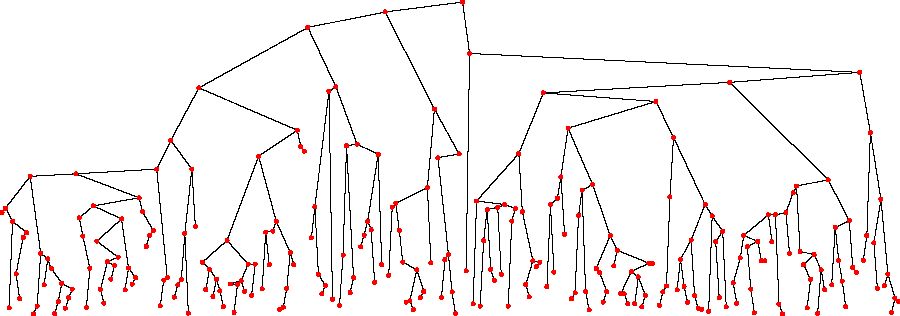
\includegraphics[scale=0.90909]{images/tree3-thick}\end{center}
  \maketitle
}}
\thetitlepage

\cleardoublepage
%
%% blank page behind title page
%\ \thispagestyle{empty}\newpage
%
%\setcounter{page}{1}
%\include{ack}
%\ \thispagestyle{empty}\newpage
%\cpponly{\include{cpp-preface}
%\ \thispagestyle{empty}\newpage
%}

% Use 14pt between lines
\setlength{\baselineskip}{14pt}


%\begin{titlepage}
%\maketitle
%\end{titlepage}

%\pagestyle{empty}
%half title page
%\newpage
%
%series page
%\newpage
%
%title page
%\newpage

\addtocontents{toc}{\protect\thispagestyle{empty}} % get rid of page number
\tableofcontents
\cleardoublepage

\fancyhead[RO,LE]{} % disable section numbers, for now
\pagestyle{fancy}
\include{ack}
\thispagestyle{empty}
\cleardoublepage

\fancyhead[CE]{\small Why This Book?} % chapter title, left center
\chapter*{なぜこの本を書いたのか}
% TALK: Why This Book? はどういう意図か?例:「なぜこの本はあるのか?」「なぜこの本を筆者が書いたのか?」「なぜこの本を読者が読むのか?」(内容的に最後のものではなさそう。)
\addcontentsline{toc}{chapter}{なぜこの本を書いたのか}

いろいろなデータ構造の入門書がある。できの良いものもある。ほとんどはタダではないので、コンピュータサイエンスを学ぶ学部生はデータ構造の本にお金を払うだろう。

オンラインで公開されているデータ構造の本もある。名作もあるのだが古くなってきているものが多い。ほとんどは著者や出版社が更新をやめるときに無料になったものである。これらの本は次の理由からふつうは内容を更新できない。(1)著者または出版社が著作権を持っていて、いずれかの許可を得られないため。(2)書籍の\emph{ソースコード}が提供されていないため。つまり、本のWord、WordPerfect、FrameMaker、または\LaTeX{}ソースコードが手に入らない、またはそれを扱えるソフトウェアのバージョンが手に入らないため。

このプロジェクトの目標は、コンピュータサイエンスを専攻する学部生が負担するデータ構造の入門書代をゼロにすることだ。そのため、オープンソース\ejindex{Open Source}{おーぷんそーす@オープンソース}のソフトウェアプロジェクトのようにこの本を作ることにした。この本の\LaTeX{}ソース、\lang{}ソース、およびビルドスクリプトを、著者のWebサイト\footnote {\url{http://opendatastructures.org}}あるいは信頼できるソースコード管理サイト\footnote {\url{https://github.com/patmorin/ods}}からダウンロードできる。\footnote {訳注:日本語版のWebサイトは\url{https://sites.google.com/view/open-data-structures-ja}} である。また、日本語版のソースコードは\url{https://github.com/spinute/ods}にある。

% TODO: 書籍版は Creative Commons ではないので、書籍版のこの部分ではそのことを注記したほうがよさそう
ソースコードはCreative Commons Attributionライセンスで公開されている。つまり誰でも自由にコピー、配布、送信してよい。内容を取り入れて別の何かを作ってもよい。そしてそれを商業的に利用してもよい。唯一の条件は\emph{attribution}である。つまり派生した作品が\url{opendatastructures.org}のコードやテキストを含むことを明記しなければならない。

ソースコード管理システム\texttt{git} \index{git@\texttt{git}}を使って、誰でも本書の修正案を送れる。本のソースをフォークして別バージョンを作ることもできる。(例えば別のプログラミング言語を使う版を作れる。)こうしたやり方で、私のやる気や興味が衰えた後でもこの本が役立つものであり続けることを望んでいる。

\cleardoublepage

\cpponly{
  \include{cpp-preface}
  \cleardoublepage
}

\fancyhead[CE]{\small\nouppercase{\leftmark}} % chapter title, left center
\fancyhead[CO]{\small\rightmarktitle} % section title, right center
\fancyhead[RO,LE]{\small\rightmarksection}

%% Include all the chapters one at a time
\include{intro-lang}
\include{arrays-lang}
\include{linkedlists-lang}
\include{skiplists-lang}
\include{hashing-lang}
\include{binarytrees-lang}
\include{rbs-lang}
\include{scapegoat-lang}
\include{redblack-lang}
\include{heaps-lang}
\include{sorting-lang}
\include{graphs-lang}
\include{integers-lang}
\include{btree-lang}

%% Turn off section numbers for remainder of document
\fancyhead[RO]{} % section number on the outside
\fancyhead[LE]{} % section number on the outside
\renewcommand{\chaptermark}[1]{\markboth{#1}{}} 
\renewcommand{\sectionmark}[1]{\markright{#1}} 
\fancyhead[CO]{\small\nouppercase\rightmark}

\cleardoublepage
\addcontentsline{toc}{chapter}{Bibliography}
\bibliographystyle{abbrvurl}
\bibliography{ods,odsproc}

\cleardoublepage
\addcontentsline{toc}{chapter}{Index}
\printindex

\end{document}

